\documentclass{article}

\usepackage{arxiv}

\usepackage[utf8]{inputenc} % allow utf-8 input
\usepackage[T1]{fontenc}    % use 8-bit T1 fonts
\usepackage{hyperref}       % hyperlinks
\usepackage{url}            % simple URL typesetting
\usepackage{booktabs}       % professional-quality tables
\usepackage{microtype}      % microtypography
\usepackage{graphicx}
\usepackage{natbib}         % citations
\usepackage{placeins}       % \FloatBarrier to keep floats near their section
\usepackage{tikz}
\usepackage{pgfplots}
\pgfplotsset{compat=1.18}
\usetikzlibrary{arrows.meta, positioning, shapes.geometric, fit, backgrounds}

\title{When Vowels Don't Help: Empirical Limits of Vowel--Consonant Separation for Compression and LLM Pipelines}

\author{
	Mohammed Abdul Moid\thanks{Corresponding author.} \\
	Department of Computer Science Engineering \\
	Muffakham Jah College of Engineering and Technology \\
	Hyderabad, India \\
	\texttt{160423733076@gmail.com} \\
	\And
	Syeda Fayeqa Nabeel \\
	Department of Computer Science Engineering \\
	Muffakham Jah College of Engineering and Technology \\
	Hyderabad, India \\
	\texttt{160423733062@gmail.com} \\
	\And
	Mohammed Afeefuddin \\
	Department of Computer Science Engineering \\
	Muffakham Jah College of Engineering and Technology \\
	Hyderabad, India \\
	\texttt{160423733101@gmail.com} \\
	\And
	Syed Liyaqat Ahmed Ali \\
	Department of Computer Science Engineering \\
	Muffakham Jah College of Engineering and Technology \\
	Hyderabad, India \\
	\texttt{160423733102@gmail.com} \\
	\And
	Mohammed Abdul Lateef \\
	Department of Computer Science Engineering \\
	Muffakham Jah College of Engineering and Technology \\
	Hyderabad, India \\
	\texttt{160423733099@gmail.com} \\
}

\renewcommand{\shorttitle}{When Vowels Don't Help}

\hypersetup{
pdftitle={When Vowels Don't Help: Empirical Limits of Vowel-Consonant Separation for Compression and LLM Pipelines},
pdfsubject={cs.CL, cs.IR},
pdfauthor={Mohammed Abdul Moid, Syeda Fayeqa Nabeel, Mohammed Afeefuddin, Syed Liyaqat Ahmed Ali, Mohammed Abdul Lateef},
pdfkeywords={text compression, tokenization, embeddings, RAG, negative results},
}

\begin{document}
\maketitle

\begin{abstract}
We study a simple linguistic transform that separates English vowels from consonants (MVD, Maharashtran Vowel Disappearance) and ask whether it helps three common goals: reversible representation, lossless compression with standard codecs, and cheaper LLM/RAG pipelines via lossy vowel dropping. The reversible split works. Lossless MVD serialization plus gzip/bz2/zlib is \emph{worse} than compressing raw text (about $-120\%$ relative improvement on short synthetic corpora; still strongly negative on real books). Lossy vowel dropping before gzip \emph{does} help: about $+14\%$ mean savings on synthetic text and $\mathbf{+20.5\%}$ mean savings on real public-domain prose at $\geq 200$ KB. The same lossy transform fails for RAG-relevant proxies: tiktoken (\texttt{cl100k\_base}) token counts \emph{increase} by an unweighted mean of 76.8\%, and sentence-transformer cosine similarity collapses to 0.17 (96.7\% of pairs below 0.6). We conclude that vowel dropping is a narrow byte-level compression trick, not a path to LLM token or embedding efficiency. Byte savings do not transfer to BPE tokenizers or pretrained embedders that rely on recognizable subword units.
\end{abstract}

\keywords{text compression \and tokenization \and embeddings \and retrieval-augmented generation \and negative results}

\section{Introduction}

Natural language is redundant \citep{shannon1948}. Vowels are frequent, often predictable, and, under a na\"ive reading, candidates for removal or relocation. That intuition appears in shorthand systems, abjad scripts, and informal ``disemvoweling.'' In systems research it reappears as a hope that a language-aware preprocess might:

\begin{enumerate}
	\item reorganize text for better lossless compression,
	\item reduce LLM token counts (and thus RAG cost), or
	\item preserve enough semantics for embedding-based retrieval after aggressive shortening.
\end{enumerate}

We implement a minimal, auditable transform, \textbf{MVD}, and test these hopes with fixed protocols and frozen data. We do \emph{not} claim a new cipher, a production compressor, or a RAG system. We claim measurements.

\paragraph{Contributions.}

\begin{enumerate}
	\item A reversible vowel/consonant/mask transform with full round-trip tests and microbenchmarks.
	\item Evidence that \textbf{lossless} stream separation + standard codecs fails under our MVDC serialization (header/structure overhead dominates).
	\item Evidence that \textbf{lossy} vowel dropping before gzip yields consistent savings on both synthetic and real English text ($\sim$20\% at book scale).
	\item A decisive \textbf{negative} result for LLM/RAG proxies: token counts rise; embedding similarity collapses, with a shared mechanism (BPE / subword opacity of consonant skeletons).
\end{enumerate}

\section{Method: MVD}
\label{sec:method}

\subsection{Reversible transform}

For ASCII vowels $\{a,e,i,o,u\}$ (both cases), MVD maps a string $S$ to:

\begin{itemize}
	\item $C$: consonant stream (all non-vowels, order preserved),
	\item $V$: ordered vowel sequence,
	\item $M$: position mask ($1$ = vowel removed).
\end{itemize}

Reconstruction is exact given $(C,V,M)$. Accented characters and non-Latin scripts are treated as consonants under the current vowel set, an intentional limitation for this study.

\subsection{Lossless packaging (MVDC)}

For lossless experiments we serialize $(C,V,M)$ as an MVDC blob: fixed header, UTF-8 consonants, 4-bit packed vowels, RLE-encoded mask. Downstream codecs: gzip, bz2, zlib.

\subsection{Lossy variant}

For lossy experiments we discard $V$ and $M$ and keep only $C$ (consonants-only text), then compress with gzip. This is \textbf{not} reversible.

\subsection{LLM / embedding probes}

\begin{itemize}
	\item \textbf{Tokens:} tiktoken \texttt{cl100k\_base} on original vs.\ consonants-only text.
	\item \textbf{Embeddings:} \texttt{all-MiniLM-L6-v2}, cosine similarity of original vs.\ consonants-only pairs.
\end{itemize}

Decision thresholds (set before measuring Stage A): mean token reduction $\geq 15\%$; mean cosine $\geq 0.85$; rate of pairs with similarity $< 0.6$ under 10\%. Failure of both metric families ends further RAG pipeline work.

\begin{figure}[ht]
	\centering
	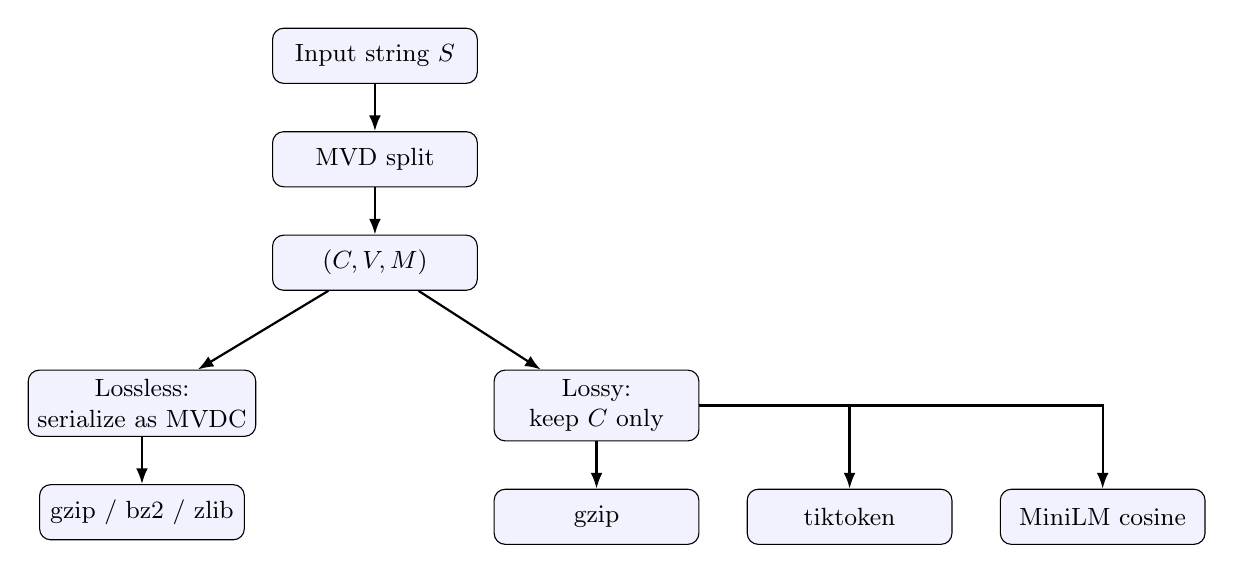
\begin{tikzpicture}[
			node distance=6mm and 6mm,
			box/.style={draw, rounded corners, align=center, font=\small, minimum height=7mm, minimum width=26mm, fill=blue!5},
			arrow/.style={-{Latex[length=2mm]}, thick}
		]
		\node[box] (input) {Input string $S$};
		\node[box, below=of input] (split) {MVD split};
		\node[box, below=of split] (cvm) {$(C, V, M)$};
		\node[box, below left=10mm and 2mm of cvm] (lossless) {Lossless:\\serialize as MVDC};
		\node[box, below right=10mm and 2mm of cvm] (lossy) {Lossy:\\keep $C$ only};
		\node[box, below=of lossless] (codec) {gzip / bz2 / zlib};
		\node[box, below=of lossy] (gzipb) {gzip};
		\node[box, right=6mm of gzipb] (tok) {tiktoken};
		\node[box, right=6mm of tok] (emb) {MiniLM cosine};

		\draw[arrow] (input) -- (split);
		\draw[arrow] (split) -- (cvm);
		\draw[arrow] (cvm) -- (lossless);
		\draw[arrow] (cvm) -- (lossy);
		\draw[arrow] (lossless) -- (codec);
		\draw[arrow] (lossy) -- (gzipb);
		\draw[arrow] (lossy.east) -| (tok.north);
		\draw[arrow] (lossy.east) -| (emb.north);
	\end{tikzpicture}
	\caption{The MVD pipeline. A string $S$ is split into consonants $C$, vowels $V$, and mask $M$. The lossless branch serializes all three (MVDC) before compression; the lossy branch keeps only $C$ and feeds three probes: byte-level compression (gzip), tokenization (tiktoken), and embedding similarity (MiniLM).}
	\label{fig:pipeline}
\end{figure}

\FloatBarrier
\section{Experiments}
\label{sec:experiments}

\subsection{Phase 0: Correctness and Speed}

Eight unit tests (reversibility, edges, case, punctuation, bitstream, vowel packing) all pass. Encode/decode at 10 KB is sub-millisecond; $\sim$1 MB round-trip is $\sim$230 ms on our test machine. The transform is space-neutral: it reorganizes characters, it does not shrink them.

\subsection{Phase 2: Compression (Synthetic)}

Five deterministic synthetic corpora (\texttt{random.seed(42)}), roughly 3--7 KB each: literature-, technical-, and news-like word bags, plus vowel-heavy and consonant-heavy bags.

\paragraph{Lossless.} Mean improvement of MVDC+codec vs.\ raw+codec across all corpora and codecs: $\mathbf{-119.78\%}$ (negative = worse). MVDC size overhead before compression ranges from $+5.8\%$ to $+116.8\%$. Modern codecs already exploit mixed-ASCII redundancy; relocating vowels into a verbose container does not help on these lengths.

\paragraph{Lossy.} Gzip on consonants-only vs.\ gzip on raw text:

\begin{table}[h]
	\caption{Lossy gzip savings on synthetic corpora (Phase 2).}
	\centering
	\begin{tabular}{lr}
		\toprule
		Corpus            & Gzip savings   \\
		\midrule
		literature-like   & $+18.9\%$      \\
		technical-like    & $+12.8\%$      \\
		news-like         & $+10.8\%$      \\
		vowel-heavy       & $+27.2\%$      \\
		consonant-heavy   & $+1.4\%$       \\
		\midrule
		\textbf{Mean}     & $\mathbf{+14.2\%}$ \\
		\bottomrule
	\end{tabular}
	\label{tab:phase2-lossy}
\end{table}

\begin{figure}[ht]
	\centering
	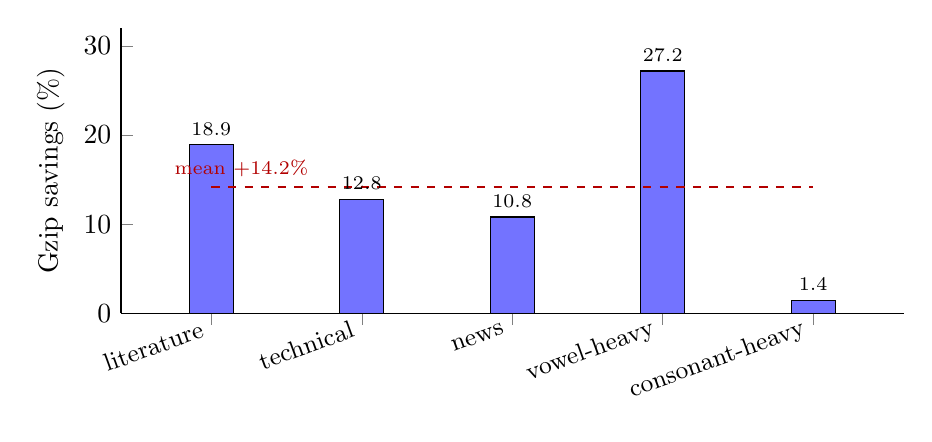
\begin{tikzpicture}
		\begin{axis}[
				ybar, bar shift=0pt,
				bar width=16pt,
				width=0.95\textwidth, height=5.2cm,
				symbolic x coords={literature, technical, news, vowel-heavy, consonant-heavy},
				xtick=data,
				x tick label style={rotate=20, anchor=east, font=\small},
				ylabel={Gzip savings (\%)},
				ymin=0, ymax=32,
				nodes near coords, every node near coord/.append style={font=\scriptsize},
				enlarge x limits=0.15,
				axis lines*=left,
			]
			\addplot[fill=blue!55] coordinates {
					(literature,18.9) (technical,12.8) (news,10.8) (vowel-heavy,27.2) (consonant-heavy,1.4)
				};
			\draw[dashed, red!70!black, thick] (axis cs:literature,14.2) -- (axis cs:consonant-heavy,14.2)
			node[pos=0.05, above, font=\scriptsize, red!70!black] {mean $+14.2\%$};
		\end{axis}
	\end{tikzpicture}
	\caption{Lossy gzip savings by synthetic corpus (Phase 2), with the dashed line marking the mean.}
	\label{fig:phase2-bar}
\end{figure}

\FloatBarrier
\subsection{Real-text compression follow-on}

To check that $+14.2\%$ was not an artifact of short word salad, we froze three public-domain sources (\emph{Pride and Prejudice}, \emph{Frankenstein}, RFC 8259), sliced UTF-8 prefixes at 50 KB / 200 KB / full (RFC is only $\sim$28 KB), and reused the Phase 2 protocol.

\begin{table}[h]
	\caption{Lossy gzip savings: synthetic vs.\ real text.}
	\centering
	\begin{tabular}{lr}
		\toprule
		Setting                    & Mean lossy gzip savings \\
		\midrule
		Synthetic (Phase 2)        & $+14.2\%$               \\
		Real, all samples ($n=7$)  & $\mathbf{+20.43\%}$     \\
		Real, $\geq 200$ KB ($n=4$)& $\mathbf{+20.47\%}$     \\
		\bottomrule
	\end{tabular}
	\label{tab:real-corpus}
\end{table}

\begin{figure}[ht]
	\centering
	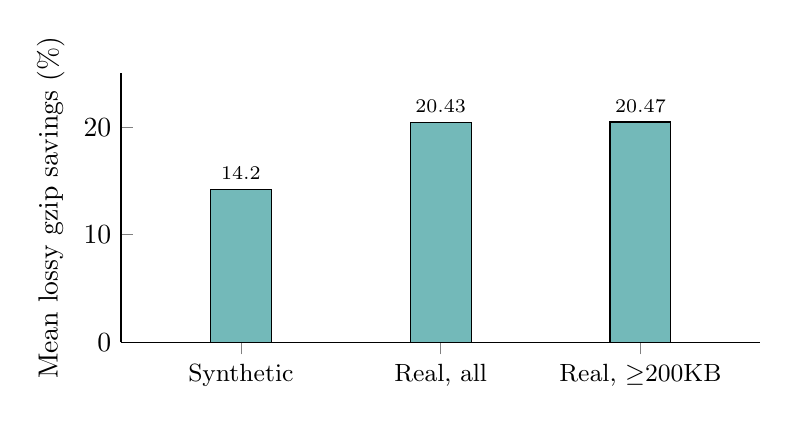
\begin{tikzpicture}
		\begin{axis}[
				ybar, bar shift=0pt,
				bar width=22pt,
				width=0.8\textwidth, height=5cm,
				symbolic x coords={Synthetic, {Real, all}, {Real, $\geq$200KB}},
				xtick=data,
				x tick label style={font=\small},
				ylabel={Mean lossy gzip savings (\%)},
				ymin=0, ymax=25,
				nodes near coords, every node near coord/.append style={font=\scriptsize},
				enlarge x limits=0.3,
				axis lines*=left,
			]
			\addplot[fill=teal!55] coordinates {
					(Synthetic,14.2) ({Real, all},20.43) ({Real, $\geq$200KB},20.47)
				};
		\end{axis}
	\end{tikzpicture}
	\caption{Lossy gzip savings: synthetic word bags vs.\ real public-domain prose. Savings hold up, and slightly increase, at book scale.}
	\label{fig:real-vs-synth-bar}
\end{figure}

Pre-registered claim rule: mean lossy savings at $\geq 200$ KB $\geq 5\%$. \textbf{Claim holds.} Lossless MVDC+codec remains worse on every real sample (roughly $-45\%$ to $-75\%$ relative to raw+codec).

\FloatBarrier
\subsection{Stage A: Tokens and Embeddings}

\paragraph{Tokens} (same synthetic corpora as Phase 2):

\begin{table}[h]
	\caption{Token count change, consonants-only vs.\ original text (tiktoken \texttt{cl100k\_base}). Negative reduction \% indicates token count increased.}
	\centering
	\begin{tabular}{lr}
		\toprule
		Corpus              & Reduction \%              \\
		\midrule
		literature-like     & $-65.8\%$ (tokens up)     \\
		technical-like      & $-165.0\%$                \\
		news-like           & $-170.0\%$                \\
		vowel-heavy         & $+23.3\%$ (only win)      \\
		consonant-heavy     & $-6.6\%$                  \\
		\midrule
		\textbf{Unweighted mean} & $\mathbf{-76.8\%}$    \\
		\bottomrule
	\end{tabular}
	\label{tab:tokens}
\end{table}

\begin{figure}[ht]
	\centering
	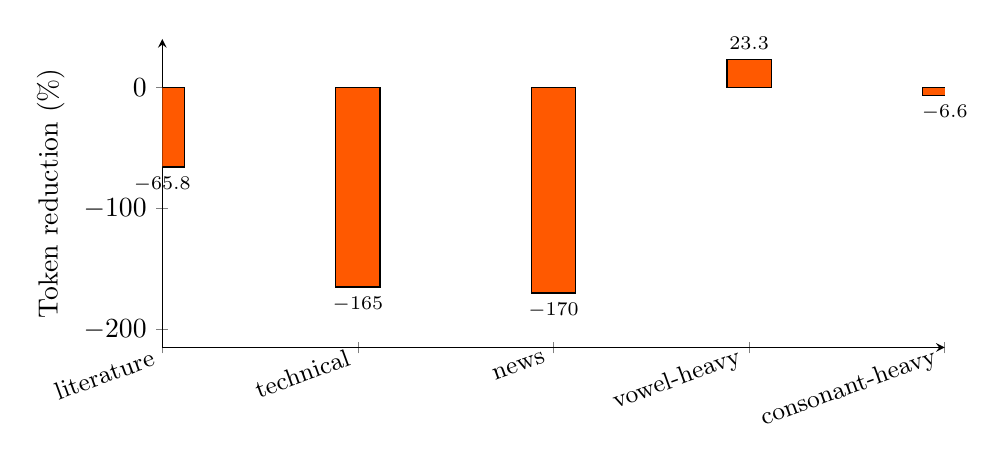
\begin{tikzpicture}
		\begin{axis}[
				ybar,
				bar width=16pt,
				width=0.95\textwidth, height=5.5cm,
				symbolic x coords={literature, technical, news, vowel-heavy, consonant-heavy},
				xtick=data,
				x tick label style={rotate=20, anchor=east, font=\small},
				ylabel={Token reduction (\%)},
				ymin=-215, ymax=40,
				nodes near coords, every node near coord/.append style={font=\scriptsize},
				enlarge x limits=0.15,
				axis x line=bottom,
				axis y line=left,
			]
			\addplot[fill=orange!70!red] coordinates {
					(literature,-65.8) (technical,-165.0) (news,-170.0) (vowel-heavy,23.3) (consonant-heavy,-6.6)
				};
		\end{axis}
	\end{tikzpicture}
	\caption{Token-count change, consonants-only vs.\ original text (tiktoken \texttt{cl100k\_base}). Bars below zero mean token count \emph{increased}; only the vowel-heavy bag nets a reduction.}
	\label{fig:tokens-bar}
\end{figure}

\paragraph{Embeddings} (30 frozen sentences, $6\times5$ categories; literary/technical/news cited; vowel-/consonant-heavy synthetic):

\begin{table}[h]
	\caption{Embedding similarity, original vs.\ consonants-only (all-MiniLM-L6-v2).}
	\centering
	\begin{tabular}{lrr}
		\toprule
		Metric                              & Target       & Actual                \\
		\midrule
		Mean cosine                         & $\geq 0.85$  & $\mathbf{0.1744}$     \\
		Catastrophic rate (sim $< 0.6$)     & $< 10\%$     & $\mathbf{96.67\%}$ (29/30) \\
		\bottomrule
	\end{tabular}
	\label{tab:embeddings}
\end{table}

Both Stage A families fail by wide margins. We do not build a retrieval pipeline.

\FloatBarrier
\section{Why byte wins invert at the tokenizer}
\label{sec:why}

BPE vocabularies \citep{sennrich2016bpe} (and the MiniLM tokenizer stack) are trained on natural orthography. Common words map to few tokens; consonant skeletons (\texttt{btfl} for \emph{beautiful}) are out-of-vocabulary and fragment into more pieces. Character count falls while token count rises. The same opacity destroys embedding geometry: mean similarity is near orthogonal, with some negative pairs.

The vowel-heavy synthetic bag is the exception for tokens: enough characters disappear that even fragmented pieces can net fewer tokens, still not a general RAG strategy.

\section{Related work (positioning)}
\label{sec:related}

\begin{itemize}
	\item \textbf{Classical compression} already models English redundancy \citep{deutsch1996gzip, collet2021zstd}; language-aware preprocessors rarely beat gzip/zstd on plain text without loss or domain-specific codecs.
	\item \textbf{Prompt/context compression} (e.g., LLMLingua-style methods \citep{jiang2023llmlingua}) targets LLM cost with learned or extractive deletion, far more aggressive, and evaluated on task metrics. MVD is a weaker, linguistics-na\"ive baseline that fails the cheap proxies those systems must still beat.
	\item \textbf{Abjad / shorthand} traditions show humans can read reduced vowels in context; pretrained BPE models are not those humans.
\end{itemize}

We do not claim superiority over any production system. We report where a minimal linguistic prior helps and where it does not.

\section{Limitations}
\label{sec:limitations}

\begin{itemize}
	\item English ASCII vowels only; no multilingual evaluation.
	\item Lossy path is irreversible and unsuitable when exact text matters.
	\item Token study uses one encoding (\texttt{cl100k\_base}); one embedding model.
	\item Synthetic bags for token counting are not grammatical prose (by design, for continuity with Phase 2); embedding sentences are small-$n$ per category.
	\item Cryptographic preprocessing was specified but not measured.
	\item $\sim$20\% gzip savings is real but modest: gzip is already cheap, and dropping vowels changes the artifact.
\end{itemize}

\section{Conclusion}
\label{sec:conclusion}

MVD teaches a sharp lesson about transferring linguistic redundancy across layers of the stack:

\begin{table}[h]
	\caption{Summary of outcomes by layer.}
	\centering
	\begin{tabular}{ll}
		\toprule
		Layer                        & Outcome                    \\
		\midrule
		Reversible representation   & Works                      \\
		Lossless + gzip/bz2/zlib    & Fails (overhead)           \\
		Lossy + gzip (bytes)        & Helps ($\sim$14--20\%)     \\
		BPE token count             & Fails (tokens increase)    \\
		Embedding similarity        & Fails (near collapse)      \\
		\bottomrule
	\end{tabular}
	\label{tab:summary}
\end{table}

\begin{figure}[ht]
	\centering
	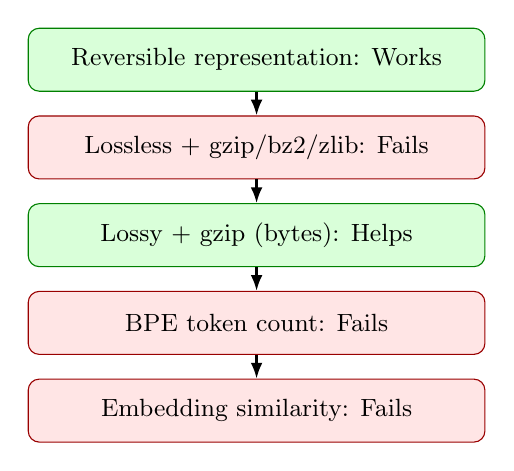
\begin{tikzpicture}[
			node distance=3mm,
			stage/.style={draw, rounded corners, align=center, font=\small, minimum height=8mm, minimum width=58mm},
			pass/.style={stage, fill=green!15, draw=green!50!black},
			fail/.style={stage, fill=red!10, draw=red!60!black},
			arrow/.style={-{Latex[length=2mm]}, thick}
		]
		\node[pass] (r1) {Reversible representation: Works};
		\node[fail, below=of r1] (r2) {Lossless + gzip/bz2/zlib: Fails};
		\node[pass, below=of r2] (r3) {Lossy + gzip (bytes): Helps};
		\node[fail, below=of r3] (r4) {BPE token count: Fails};
		\node[fail, below=of r4] (r5) {Embedding similarity: Fails};
		\draw[arrow] (r1) -- (r2);
		\draw[arrow] (r2) -- (r3);
		\draw[arrow] (r3) -- (r4);
		\draw[arrow] (r4) -- (r5);
	\end{tikzpicture}
	\caption{Outcomes by layer of the stack (same data as Table~\ref{tab:summary}).}
	\label{fig:summary-diagram}
\end{figure}

\textbf{Byte-level savings do not imply token-level or semantic-level savings.} A transform that removes predictable letters can help a byte compressor and simultaneously harm models whose units are learned subwords. For RAG cost, vowel dropping is not a viable lever under our probes. For archival or bandwidth settings that tolerate irreversible, unreadable text, consonants-only gzip remains a small, reproducible win on English prose.

\section*{Reproducibility}
\addcontentsline{toc}{section}{Reproducibility}

\noindent Code, probe scripts, and logged outputs are available at
\url{https://github.com/Morizz00/mvd-algorithm}.

\begin{table}[h]
	\caption{Artifacts and paths.}
	\centering
	\begin{tabular}{ll}
		\toprule
		Artifact                    & Path                                              \\
		\midrule
		Public repository           & \url{https://github.com/Morizz00/mvd-algorithm} \\
		Core transform              & \texttt{src/mvd\_base.py}, \texttt{phase2/mvd\_comp.py} \\
		Synthetic compression log   & \texttt{phase2\_output.log}                       \\
		Real compression            & \texttt{phase2/real\_corpus\_probe.py}, \texttt{phase2\_real\_corpus\_output.log}, \texttt{data/real/} \\
		Token / embedding probes    & \texttt{phase3/}, \texttt{phase3\_token\_output.log}, \texttt{phase3\_embedding\_output.log} \\
		Internal writeups           & \texttt{docs/probe\_results.md}, \texttt{docs/real\_corpus\_compression.md}, \texttt{MVD\_Progress\_Report.md} \\
		\bottomrule
	\end{tabular}
	\label{tab:repro}
\end{table}

\noindent\emph{Data licensing:} \emph{Pride and Prejudice} and \emph{Frankenstein} are public-domain texts distributed by Project Gutenberg; RFC 8259 is redistributed under the IETF Trust's copyright policy for RFC documents. The synthetic news-derived sentences in \texttt{phase3/sentences.json} are excluded from the public release pending a separate licensing review.

\section*{Acknowledgments}
\addcontentsline{toc}{section}{Acknowledgments}

We thank Nuzhath Begum, who did not propose MVD but whose offhand remark inspired us to explore this direction in the first place.

\bibliographystyle{unsrtnat}
\bibliography{references}

\end{document}
